\documentclass[12pt,a4paper]{article}

\usepackage[utf8]{inputenc}
\usepackage[T2A]{fontenc}
\usepackage[ukrainian]{babel}
\usepackage{geometry}
\geometry{
    left=2cm,
    right=2cm,
    top=2cm,
    bottom=2cm
}

\usepackage[table]{xcolor}
\usepackage{amsmath}
\usepackage{graphicx}
\usepackage{subcaption}
\usepackage{multirow}
\usepackage{makecell}
\usepackage{pdflscape}
\usepackage{amsfonts}
\usepackage{array}
\newcolumntype{C}[1]{>{\centering\arraybackslash}m{#1}}

\usepackage[
  unicode,
  pdftitle={ІО-41, Давидчук А.М., Алгоритми та методи обчислень, Лабораторна робота №1},
  pdfauthor={Давидчук Артем},
  pdfsubject={Алгоритми та методи обчислень}
]{hyperref}

\usepackage{minted}

\usemintedstyle{vs}
\setminted{linenos, breaklines, frame=single, fontsize=\small}

\RecustomVerbatimCommand{\VerbatimInput}{VerbatimInput}{
    breaklines=true,
    breaksymbolleft={}
}

\begin{document}


    \begin{titlepage}

        \begin{center}
\includegraphics[width=0.7\textwidth]{../../../TITLES/letterhead.png}\end{center}

        \begin{center}
            \large Національний технічний університет України\\
            «Київський політехнічний інститут імені Ігоря Сікорського»\\[1em]
            Факультет інформатики та обчислювальної техніки\\
            Кафедра обчислювальної техніки
        \end{center}

        \vfill

        \begin{center}
            \textbf{\LARGE Алгоритми та методи обчислень}\\[2em]
            \textbf{\Large Лабораторна робота №1}\\[0.5em]
            «Поняття алгоритму. Задавання алгоритмів у вигляді блок-схем»
        \end{center}

        \vfill

        \begin{flushright}
            Виконав: студент 1 курсу ФІОТ, гр. ІО-41\\
            \textit{Давидчук А. М.}\\
            Залікова книжка № 4106\\[1em]
            Перевірив: \textit{Порєв В.\,М.}
        \end{flushright}

        \vfill

        \begin{center}Київ --- 2026\end{center}

    \end{titlepage}

    \noindent
    \textbf{\underline{Тема:}} «Поняття алгоритму. Задавання алгоритмів у вигляді блок-схем» .

    \vspace{1em}

    \noindent
    \textbf{\underline{Мета:}} Навчитися створювати блок-схеми лінійного алгоритму; розгалуженого
                                алгоритму та циклічного алгоритму за допомогою редактора блок-схем afce
                                або іншого довільного редактора.

    \begin{center} \textbf{\large Хід роботи} \end{center}

    \noindent
    Мій порядковий номер у списку групи: 6, звідси я маю реалізувати такий варіант:

    \begin{figure}[h!]
        \centering
        
\includegraphics[width=0.8\linewidth]{media/task.png}
        \caption{Варіант функцій для 6 варіанту}
    \end{figure}

    де функцію $Y1$ я маю обчислити за допомогою лінійного алгоритму, $y$ -- розгалуженим, $f$ -- циклічним (детермінованим циклом).

    \vspace{1em}

    \noindent
    Блок-схема лінійного алгоритму обчислення функції $Y1 = (d \cdot a)^b + (b \cdot c)^{\frac{1}{d}}$:

    \begin{figure}[h!]
        \centering
        \includegraphics[width=0.2\linewidth]{media/linear_alg1.pdf}
    \end{figure}

    \newpage

    \begin{figure}[h!]
        \centering
        \includegraphics[width=0.23\linewidth]{media/linear_alg2.pdf}
    \end{figure}

    Тут функція \texttt{pow(x, y)} -- функція піднесення числа $x$ до степеню $y$:
    
    \[
    \texttt{pow(x, y)} = x^y
    \]

    Щодо недоліків цього алгоритму: він не враховує нульове значення змінної $d$ що може викликати помилку під час обчислення $1 / d$ -- запобігти помилці можна лише якщо додати умову перевірки цієї змінної що не є можливим в данному випадку, тому що при такій модифікації алгоритм перестане бути лінійним, і стане тим, що розгалужується. Тому правильність виконання алгоритму залежить від вводу користувача.

    Також можна було б зазначити, якби $d$ змінна була парною, а вираз $b \cdot c$ був від'ємним, або $b$ парне, і $d \cdot a$ -- від'ємне, і виходить при цьому виникала б помилка, коли ми хочемо взяти корінь із парним степенем від'ємного числа -- але ми працюватимемо не на дійсній множині чисел, а на комплексній, яка запобігатиме таким помилкам невизначеності. Звідси також можна зробити висновок, що функція $Y1$ завжди буде належати до множини комплексних чисел (є комплексним числом).

    \newpage

    \noindent
    Блок-схема розгалуженого алгоритму обчислення функції $y = \dfrac{4r - rx}{4x - rx}$:

    \begin{figure}[h!]
        \centering
        \includegraphics[width=0.7\linewidth]{media/branched_alg.pdf}
    \end{figure}

    Тут бачимо, що знаменник дорівнює нулю, коли $x = 0$ або $r = 4$, бо $4x - rx = x(4-r)$ прирівнюючи яке до нуля, та розв'язавши отримаємо 2 рішення. Якщо $x = 0$ або $r = 4$, то виводиться повідомлення про помилку ділення на нуль.

    \newpage

    \noindent
    Блок-схема циклічного алгоритму обчислення функції $\displaystyle f = \sum_{a=0}^{n}\left(\sum_{b=0}^{p}\left(a^{b} + b^{a}\right)\right)$:

    \begin{figure}[h!]
        \centering
        \includegraphics[width=0.72\linewidth]{media/cyclic_alg.pdf}
    \end{figure}

    Тут потрібно зазначити, що ми приймаємо $0^0 = 1$, тобто

    \[
    \texttt{pow(0, 0)} = 1
    \]

    Також зазначимо, що кількість ітерація від початку відома (її кількість вводиться користувачем) -- звідси всі цикли, які присутні в цьому алгоритмі -- детерміновані. Це було видно на блок-схемі, коли для заголовку
    детермінованого цилку використовувався гексагон.

    \vspace{1em}

    Для реалізації алгоритмів та GUI середовища я використовуватиму мову програмування Python і інструмент Tkinter та бібліотеку customtkinter.

    \vspace{1em}

    \noindent
    \textbf{\underline{Програмний код для реалізації лінійного алгоритму (\texttt{src/linear\_alg.py})}}:

    \begin{minted}{python3}
from __future__ import annotations

def linear_alg(*, a: int | float | complex, b: int | float | complex, c: int | float | complex, d: int | float | complex) -> complex:
    """
    Обчислює функцію Y1 = (d*a)^b + (b*c)^(1/d)

    a, b, c, d можуть бути int/float/complex.
    Під час обчислень трактуються як комплексні.
    Обмеження яке в алгоритмі не враховується: d != 0.
    """

    t1 = d * a
    t2 = b * c

    p = 1 / d

    g1 = t1 ** b
    g2 = t2 ** p

    Y1 = g1 + g2

    return complex(Y1)
    \end{minted}

    \noindent
    \textbf{\underline{Програмний код для реалізації розгалуженого алгоритму (\texttt{src/branched\_alg.py})}}:

    \begin{minted}{python3}
from __future__ import annotations

def branched_alg(*, r: int | float | complex, x: int | float | complex) -> complex:
    """
    Обчислює функцію y = (4*r - r*x) / (4*x - r*x)

    r, x можуть бути int/float/complex.
    Під час обчислень трактуються як комплексні.
    Обмеження яке в алгоритмі враховується: x != 0 та r != 4.
    """

    if (x == 0) or (r == 4):

        raise ZeroDivisionError("x != 0 and r != 4!")

    t1 = r * x

    g1 = 4*r - t1
    g2 = 4*x - t1

    y = g1 / g2

    return complex(y)
    \end{minted}

    \noindent
    \textbf{\underline{Програмний код для реалізації циклічного алгоритму (\texttt{src/cyclic\_alg.py})}}:

    \begin{minted}{python3}
from __future__ import annotations

def cyclic_alg(*, n: int, p: int) -> int:

    f: int = 0

    if (
        isinstance(n, bool) or not isinstance(n, int)    # Число n строго є типом int (і не bool зокрема)
        or isinstance(p, bool) or not isinstance(p, int) # Число p строго є типом int (і не bool зокрема)
    ):

        raise TypeError("n and p must be int (not float/complex/bool)")

    if (n < 0) or (p < 0):

        raise ValueError("n and p must be non-negative integers (>= 0)")

    for a in range(n+1):

        for b in range(p+1):

            t1 = a**b
            t2 = b**a

            f += t1 + t2

    return f
    \end{minted}

    \noindent
    \textbf{\underline{Програмний код основної програми (\texttt{app.py})}}:

    \begin{minted}{python3}
from __future__ import annotations

import json
import re
import tkinter as tk
from dataclasses import dataclass
from pathlib import Path
from tkinter import filedialog
from typing import Callable

import customtkinter as ctk

from src.branched_alg import branched_alg
from src.cyclic_alg import cyclic_alg
from src.linear_alg import linear_alg

MAIN_THEME: dict[str, str] = {
    "bg": "#000000",
    "topbar": "#000000",
    "panel": "#090909",
    "surface": "#111111",
    "surface_soft": "#1B1B1B",
    "text": "#F5F7FA",
    "muted": "#97A1AD",
    "accent": "#29A8FF",
    "accent_hover": "#44B4FF",
    "accent_text": "#06121B",
    "segment": "#131313",
    "segment_hover": "#1E1E1E",
    "segment_active": "#1F2D3C",
    "error": "#FF5B71",
}

INT_PATTERN = re.compile(r"^[+-]?\d+$")
EPSILON = 1e-12

@dataclass(frozen=True)
class PageConfig:
    page_id: str
    nav_title: str
    title: str
    subtitle: str
    fields: tuple[str, ...]
    parser: Callable[[dict[str, str]], dict[str, object]]
    compute: Callable[..., object]


def parse_complex_fields(raw_values: dict[str, str]) -> dict[str, complex]:
    parsed: dict[str, complex] = {}
    for key, raw in raw_values.items():
        value = raw.strip()
        if not value:
            raise ValueError(f"'{key}' is required")

        try:
            parsed[key] = complex(value)
        except ValueError as exc:
            raise ValueError(
                f"'{key}' must be a complex-compatible string (examples: '1', '2.5', '1+2j')"
            ) from exc
    return parsed


def parse_cyclic_fields(raw_values: dict[str, str]) -> dict[str, int]:
    parsed: dict[str, int] = {}
    for key in ("n", "p"):
        raw = raw_values[key].strip()
        if not raw:
            raise ValueError(f"'{key}' is required")
        if not INT_PATTERN.fullmatch(raw):
            raise TypeError(f"'{key}' must be an integer string (for example: '0', '5', '12')")

        value = int(raw)
        if value < 0:
            raise ValueError(f"'{key}' must be >= 0")
        parsed[key] = value
    return parsed


def _normalize_zero(value: float) -> float:
    return 0.0 if abs(value) < EPSILON else value


def _format_real(value: float) -> str:
    normalized = _normalize_zero(value)
    if float(normalized).is_integer():
        return str(int(normalized))
    return f"{normalized:.12g}"


def format_output_value(value: object) -> str:
    if isinstance(value, complex):
        real = _normalize_zero(float(value.real))
        imag = _normalize_zero(float(value.imag))

        if imag == 0.0:
            return _format_real(real)

        sign = "+" if imag >= 0 else "-"
        return f"{_format_real(real)} {sign} {_format_real(abs(imag))}j"

    if isinstance(value, float):
        return _format_real(value)

    return str(value)


class AlgorithmPage(ctk.CTkFrame):
    def __init__(
        self,
        master: ctk.CTkFrame,
        config: PageConfig,
        fonts: dict[str, ctk.CTkFont],
    ) -> None:
        super().__init__(master, corner_radius=0)
        self.config_data = config
        self.fonts = fonts
        self.entries: dict[str, ctk.CTkEntry] = {}
        self.field_labels: list[ctk.CTkLabel] = []
        self.result_var = tk.StringVar(value="Ready")
        self.error_var = tk.StringVar(value="")

        self.grid_columnconfigure(0, weight=1)

        self._build_header()
        self._build_form()
        self._build_actions()
        self._build_output()

    def _build_header(self) -> None:
        self.header_card = ctk.CTkFrame(self, corner_radius=14, border_width=1)
        self.header_card.grid(row=0, column=0, sticky="ew", pady=(0, 14))
        self.header_card.grid_columnconfigure(0, weight=1)

        self.title_label = ctk.CTkLabel(
            self.header_card,
            text=self.config_data.title,
            anchor="w",
            font=self.fonts["title"],
        )
        self.title_label.grid(row=0, column=0, sticky="ew", padx=20, pady=(14, 4))

        self.subtitle_label = ctk.CTkLabel(
            self.header_card,
            text=self.config_data.subtitle,
            anchor="w",
            font=self.fonts["subtitle"],
        )
        self.subtitle_label.grid(row=1, column=0, sticky="ew", padx=20, pady=(0, 12))

    def _build_form(self) -> None:
        self.form_card = ctk.CTkFrame(self, corner_radius=14, border_width=1)
        self.form_card.grid(row=1, column=0, sticky="ew", pady=(0, 14))
        self.form_card.grid_columnconfigure(1, weight=1)

        for row, field_name in enumerate(self.config_data.fields):
            label = ctk.CTkLabel(
                self.form_card,
                text=f"{field_name}:",
                width=42,
                anchor="w",
                font=self.fonts["label"],
            )
            label.grid(row=row, column=0, sticky="w", padx=(20, 12), pady=9)
            self.field_labels.append(label)

            entry = ctk.CTkEntry(
                self.form_card,
                height=38,
                corner_radius=10,
                font=self.fonts["body"],
            )
            entry.grid(row=row, column=1, sticky="ew", padx=(0, 20), pady=9)
            self.entries[field_name] = entry

    def _build_actions(self) -> None:
        self.actions = ctk.CTkFrame(self, fg_color="transparent")
        self.actions.grid(row=2, column=0, sticky="ew", pady=(0, 10))
        self.actions.grid_columnconfigure((0, 1), weight=1)

        self.compute_button = ctk.CTkButton(
            self.actions,
            text="Compute",
            height=42,
            corner_radius=11,
            font=self.fonts["button"],
            command=self.compute,
        )
        self.compute_button.grid(row=0, column=0, sticky="ew", padx=(0, 7))

        self.load_button = ctk.CTkButton(
            self.actions,
            text="Load JSON",
            height=42,
            corner_radius=11,
            font=self.fonts["button"],
            command=self.load_json,
        )
        self.load_button.grid(row=0, column=1, sticky="ew", padx=(7, 0))

    def _build_output(self) -> None:
        self.output_card = ctk.CTkFrame(self, corner_radius=14, border_width=1)
        self.output_card.grid(row=3, column=0, sticky="ew")
        self.output_card.grid_columnconfigure(0, weight=1)

        self.result_title = ctk.CTkLabel(
            self.output_card,
            text="Result",
            anchor="w",
            font=self.fonts["label"],
        )
        self.result_title.grid(row=0, column=0, sticky="ew", padx=20, pady=(14, 4))

        self.result_label = ctk.CTkLabel(
            self.output_card,
            textvariable=self.result_var,
            anchor="w",
            font=self.fonts["result"],
        )
        self.result_label.grid(row=1, column=0, sticky="ew", padx=20, pady=(0, 6))

        self.error_label = ctk.CTkLabel(
            self.output_card,
            textvariable=self.error_var,
            anchor="w",
            justify="left",
            wraplength=860,
            font=self.fonts["body"],
        )
        self.error_label.grid(row=2, column=0, sticky="ew", padx=20, pady=(0, 14))

    def apply_theme(self, palette: dict[str, str]) -> None:
        self.configure(fg_color=palette["bg"])

        for card in (self.header_card, self.form_card, self.output_card):
            card.configure(
                fg_color=palette["panel"],
                border_color=palette["surface_soft"],
            )

        self.title_label.configure(text_color=palette["text"])
        self.subtitle_label.configure(text_color=palette["muted"])

        for label in self.field_labels:
            label.configure(text_color=palette["muted"])

        for entry in self.entries.values():
            entry.configure(
                fg_color=palette["surface"],
                border_color=palette["surface_soft"],
                text_color=palette["text"],
                placeholder_text_color=palette["muted"],
            )

        self.compute_button.configure(
            fg_color=palette["accent"],
            hover_color=palette["accent_hover"],
            text_color=palette["accent_text"],
        )
        self.load_button.configure(
            fg_color=palette["segment"],
            hover_color=palette["segment_hover"],
            text_color=palette["text"],
        )

        self.result_title.configure(text_color=palette["muted"])
        self.result_label.configure(text_color=palette["text"])
        self.error_label.configure(text_color=palette["error"])

    def _collect_raw_values(self) -> dict[str, str]:
        return {key: entry.get() for key, entry in self.entries.items()}

    def _show_result(self, value: object) -> None:
        self.result_var.set(format_output_value(value))
        self.error_var.set("")

    def _show_error(self, error: Exception | str) -> None:
        self.result_var.set("No result")
        self.error_var.set(f"Error: {error}")

    def _set_entries_from_dict(self, values: dict[str, str]) -> None:
        for key, entry in self.entries.items():
            entry.delete(0, tk.END)
            entry.insert(0, values[key])

    def load_json(self) -> None:
        path = filedialog.askopenfilename(
            title="Select JSON file",
            filetypes=[("JSON files", "*.json"), ("All files", "*.*")],
        )
        if not path:
            return

        try:
            raw_data = Path(path).read_text(encoding="utf-8")
            loaded = json.loads(raw_data)

            if not isinstance(loaded, dict):
                raise ValueError("JSON root must be an object")

            expected_keys = set(self.config_data.fields)
            actual_keys = set(loaded.keys())
            if actual_keys != expected_keys:
                raise ValueError(f"Expected keys exactly: {sorted(expected_keys)}")

            for key in self.config_data.fields:
                if not isinstance(loaded[key], str):
                    raise TypeError(f"JSON value for '{key}' must be a string")

            prepared = {key: loaded[key] for key in self.config_data.fields}
            self._set_entries_from_dict(prepared)
            self.error_var.set("")
            self.result_var.set("JSON loaded. Press Compute.")
        except Exception as exc:
            self._show_error(exc)

    def compute(self) -> None:
        try:
            raw_values = self._collect_raw_values()
            parsed = self.config_data.parser(raw_values)
            result = self.config_data.compute(**parsed)
            self._show_result(result)
        except Exception as exc:
            self._show_error(exc)


class AlgorithmsApp(ctk.CTk):
    def __init__(self) -> None:
        super().__init__()
        ctk.set_appearance_mode("dark")

        self.title("AlgorithmsDemoApp")
        self.resizable(False, False)
        self.geometry("100x500")
        self.minsize(780, 680)

        self.current_page = "linear_alg"
        self.nav_buttons: dict[str, ctk.CTkButton] = {}
        self.pages: dict[str, AlgorithmPage] = {}

        self.fonts: dict[str, ctk.CTkFont] = {
            "title": ctk.CTkFont(family="Segoe UI", size=27, weight="bold"),
            "subtitle": ctk.CTkFont(family="Segoe UI", size=13),
            "label": ctk.CTkFont(family="Segoe UI", size=13, weight="bold"),
            "body": ctk.CTkFont(family="Segoe UI", size=12),
            "button": ctk.CTkFont(family="Segoe UI", size=12, weight="bold"),
            "result": ctk.CTkFont(family="Consolas", size=18, weight="bold"),
            "nav": ctk.CTkFont(family="Segoe UI", size=12, weight="bold"),
        }

        self.page_configs: tuple[PageConfig, ...] = (
            PageConfig(
                page_id="linear_alg",
                nav_title="Linear",
                title="Linear Algorithm",
                subtitle="Y1 = (d*a)^b + (b*c)^(1/d)",
                fields=("a", "b", "c", "d"),
                parser=parse_complex_fields,
                compute=linear_alg,
            ),
            PageConfig(
                page_id="branched_alg",
                nav_title="Branched",
                title="Branched Algorithm",
                subtitle="y = (4*r - r*x) / (4*x - r*x)",
                fields=("r", "x"),
                parser=parse_complex_fields,
                compute=branched_alg,
            ),
            PageConfig(
                page_id="cyclic_alg",
                nav_title="Cyclic",
                title="Cyclic Algorithm",
                subtitle="f = sum(a^b + b^a), for a in [0..n], b in [0..p]",
                fields=("n", "p"),
                parser=parse_cyclic_fields,
                compute=cyclic_alg,
            ),
        )

        self.grid_columnconfigure(0, weight=1)
        self.grid_rowconfigure(1, weight=1)

        self._build_topbar()
        self._build_pages()
        self._apply_theme()
        self.show_page(self.current_page)

    def _build_topbar(self) -> None:
        self.topbar = ctk.CTkFrame(self, corner_radius=0)
        self.topbar.grid(row=0, column=0, sticky="ew")
        self.topbar.grid_columnconfigure(0, weight=1)

        self.nav_frame = ctk.CTkFrame(self.topbar, fg_color="transparent")
        self.nav_frame.grid(row=0, column=0, sticky="w", padx=20, pady=(18, 12))

        for index, page in enumerate(self.page_configs):
            button = ctk.CTkButton(
                self.nav_frame,
                text=page.nav_title,
                width=110,
                height=36,
                corner_radius=10,
                font=self.fonts["nav"],
                border_width=1,
                command=lambda pid=page.page_id: self.show_page(pid),
            )
            button.grid(row=0, column=index, padx=(0, 8))
            self.nav_buttons[page.page_id] = button

    def _build_pages(self) -> None:
        self.page_host = ctk.CTkFrame(self, corner_radius=0)
        self.page_host.grid(row=1, column=0, sticky="nsew", padx=20, pady=(0, 20))
        self.page_host.grid_rowconfigure(0, weight=1)
        self.page_host.grid_columnconfigure(0, weight=1)

        for config in self.page_configs:
            page = AlgorithmPage(self.page_host, config, self.fonts)
            page.grid(row=0, column=0, sticky="nsew")
            self.pages[config.page_id] = page

    def show_page(self, page_id: str) -> None:
        self.current_page = page_id
        self.pages[page_id].tkraise()
        self._refresh_nav_buttons()

    def _refresh_nav_buttons(self) -> None:
        palette = MAIN_THEME
        for page_id, button in self.nav_buttons.items():
            if page_id == self.current_page:
                button.configure(
                    fg_color=palette["segment_active"],
                    hover_color=palette["segment_active"],
                    text_color=palette["text"],
                    border_color=palette["segment_active"],
                )
            else:
                button.configure(
                    fg_color=palette["segment"],
                    hover_color=palette["segment_hover"],
                    text_color=palette["muted"],
                    border_color=palette["surface_soft"],
                )

    def _apply_theme(self) -> None:
        palette = MAIN_THEME

        self.configure(fg_color=palette["bg"])
        self.topbar.configure(fg_color=palette["topbar"])
        self.page_host.configure(fg_color=palette["bg"])

        for page in self.pages.values():
            page.apply_theme(palette)

        self._refresh_nav_buttons()

def main() -> None:
    app = AlgorithmsApp()
    app.mainloop()

if __name__ == "__main__":
    main()
    \end{minted}

    \noindent
    Короткий опис функціоналу основної програми:

    \begin{itemize}
        \item GUI на \texttt{customtkinter} у мінімалістичному стилі (dark).
        \item 3 сторінки алгоритмів: \texttt{linear\_alg}, \texttt{branched\_alg}, \texttt{cyclic\_alg}.
        \item Для кожної сторінки: поля вводу, кнопки \texttt{Compute} і \texttt{Load JSON}, блоки результату та помилки.
        \item JSON завантажується з файлу, ключі перевіряються строго під поточний алгоритм, значення мають бути рядками.
        \item Парсинг: для \texttt{linear/branched} -- \texttt{complex(...)}, для \texttt{cyclic} -- лише \texttt{int} і умови \texttt{n,p $\ge$ 0}.
        \item Помилки не зупиняють програму: показуються як \texttt{Error: ...}.
        \item Формат виводу: \texttt{1+0j $\to$ 1}, \texttt{2.5+0j $\to$ 2.5}, інакше \texttt{n $\pm$ mj}.
    \end{itemize}

    \newpage

    \noindent
    \underline{\textbf{Скріншоти демонстрації програми:}}

    \begin{figure}[htbp]
        \centering

        \begin{subfigure}{0.42\textwidth}
            \centering
            
\includegraphics[width=\linewidth]{media/demo1.png}
        \end{subfigure}
        \begin{subfigure}{0.42\textwidth}
            \centering
            
\includegraphics[width=\linewidth]{media/demo2.png}
        \end{subfigure}

        \vspace{1mm}

        \begin{subfigure}{0.42\textwidth}
            \centering
            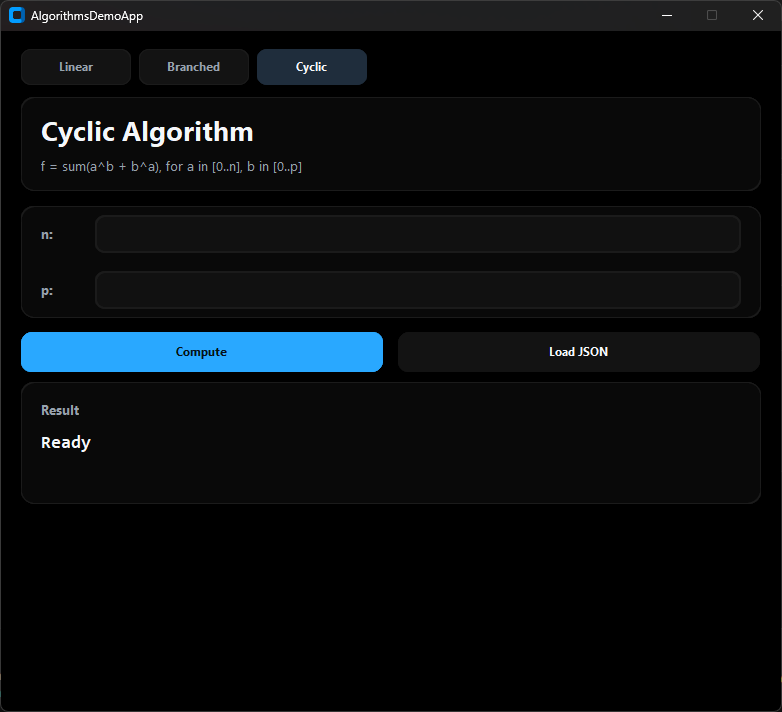
\includegraphics[width=\linewidth]{media/demo3.png}
        \end{subfigure}
        \begin{subfigure}{0.42\textwidth}
            \centering
            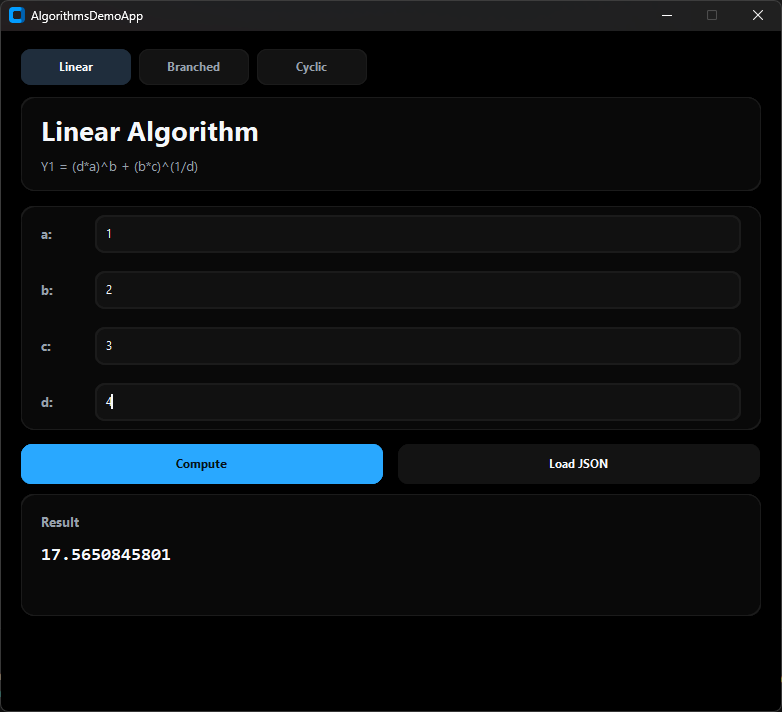
\includegraphics[width=\linewidth]{media/demo4.png}
        \end{subfigure}

        \vspace{1mm}

        \begin{subfigure}{0.42\textwidth}
            \centering
            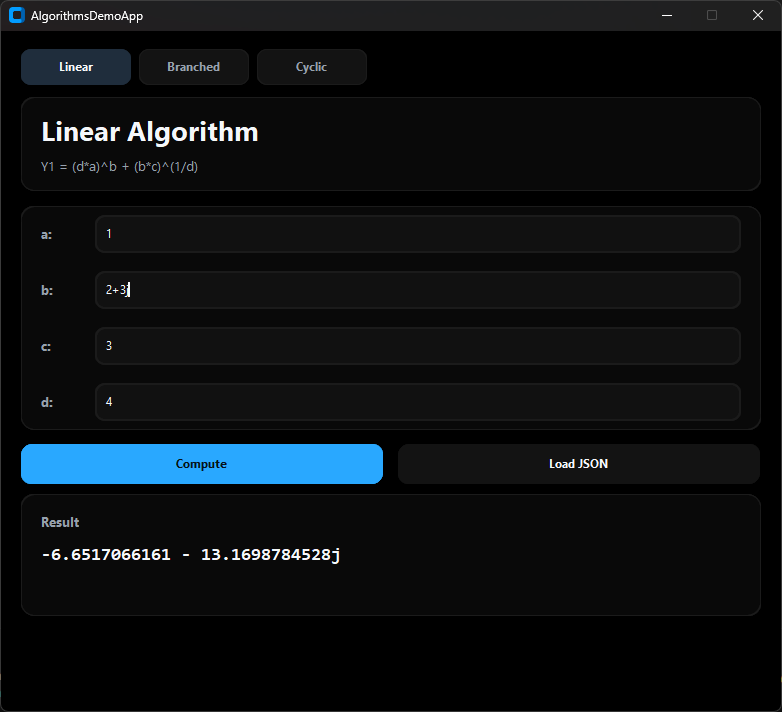
\includegraphics[width=\linewidth]{media/demo5.png}
        \end{subfigure}
        \begin{subfigure}{0.42\textwidth}
            \centering
            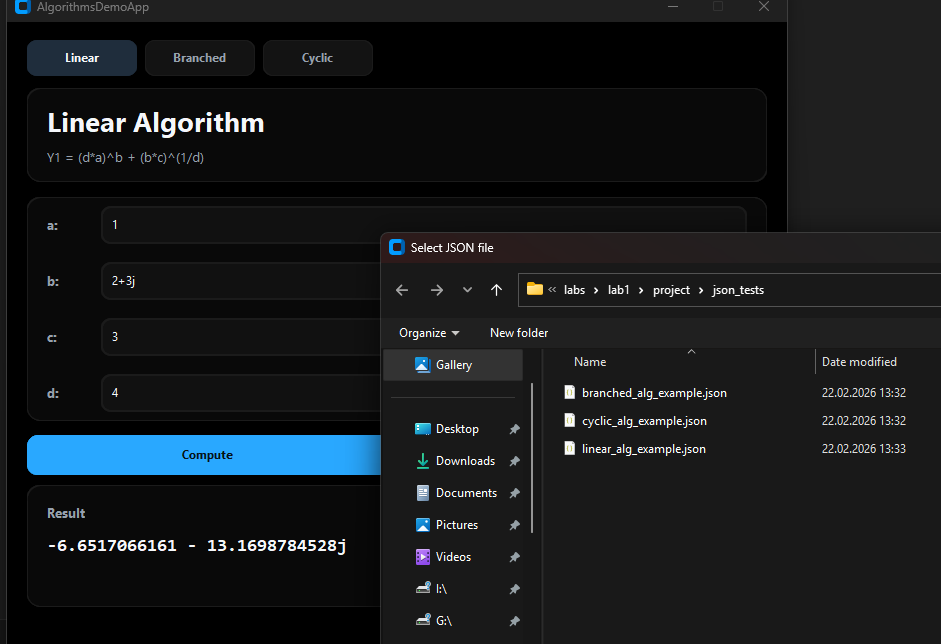
\includegraphics[width=\linewidth]{media/demo6.png}
    \end{subfigure}

    \end{figure}

    \newpage

    \begin{figure}[htbp]

        \centering

        \begin{subfigure}{0.42\textwidth}
            \centering
            
\includegraphics[width=\linewidth]{media/demo1.png}
        \end{subfigure}
        \begin{subfigure}{0.42\textwidth}
            \centering
            
\includegraphics[width=\linewidth]{media/demo2.png}
        \end{subfigure}

        \caption{Скріншоти демонстрації програми}

    \end{figure}

    \begin{center} \textbf{\large Аналіз результатів} \end{center}

    Реалізований лінійний алгоритм обчислює задану функцію $Y1$, за винятком випадку $d = 0$, коли на етапі обчислення $p=1 / d$ виникає ділення на нуль. Інших обмежень на область визначення (зокрема, пов’язаних із піднесенням до степеня) не накладається, оскільки обчислення виконуються в множині комплексних чисел $\mathbb{C}$, де операції піднесення до степеня визначені (за стандартними домовленостями реалізації комплексної степеневої функції).

    Перевірка на нульове значення змінної $d$ реалізована в основній програмі GUI, тоді як у самому лінійному алгоритмі вона відсутня. Це узгоджується з вимогами до лінійних алгоритмів (відсутність розгалужень): коректність забезпечується через попередню валідацію вхідних даних.
    
    Алгоритм уніфіковано за типом результату: він завжди повертає значення типу \texttt{complex}. Такий підхід спрощує подальшу обробку результату в GUI та робить інтерфейс однорідним. Основна програма при цьому здатна коректно інтерпретувати випадки, коли результат є дійсним (тобто має нульову уявну частину), і відрізняти їх від власне комплексних значень з ненульовою уявною частиною.

    Щодо часової складності лінійного алгоритму: кількість виконуваних кроків є сталою. Якщо припустити, що операція піднесення до степеня (функція \texttt{pow}) виконується за сталий час $O(1)$ для використаних типів даних, то загальна часова складність алгоритму становить
    \[
    T=\Theta(1)\quad (\text{тобто } T\in O(1)\ \text{і}\ T\in \Omega(1)).
    \]
    Отже, реалізований лінійний алгоритм є коректним за умови $d\neq 0$.

    Реалізований розгалужений алгоритм обчислює задану функцію $y$, за винятком випадків, коли знаменник дорівнює нулю. У даній реалізації ця умова перевіряється безпосередньо в алгоритмі, що унеможливлює некоректне введення та запобігає діленню на нуль. З аналізу виразу випливає, що нульовий знаменник виникає при $x=0$ або $r=4$, тому умови коректності мають вигляд $x\neq 0$ та $r\neq 4$.

    Як і для лінійного алгоритму, результат розгалуженого алгоритму завжди повертається у вигляді комплексного числа (\texttt{complex}). Це уніфікує формат вихідних даних і дає змогу основній програмі однаково обробляти як дійсні, так і комплексні значення, зберігаючи можливість розпізнавати випадок нульової уявної частини.

    Щодо часової складності: алгоритм виконує сталу кількість операцій (одну перевірку умови та фіксований набір арифметичних обчислень) і не містить циклів. За класичного припущення про сталу вартість арифметичних операцій часова складність становить
    \[
    T=\Theta(1)\quad (\text{тобто } T\in O(1)\ \text{і}\ T\in \Omega(1)).
    \]

    Таким чином, за виконання умов $x \neq 0$ та $r \neq 4$ розгалужений алгоритм працює коректно та забезпечує результативне обчислення заданої функції.

    Реалізований циклічний алгоритм призначений для обчислення значення функції
    \[
    f=\sum_{a=0}^{n}\left(\sum_{b=0}^{p}\left(a^{b}+b^{a}\right)\right).
    \]
    Оскільки вказаний вираз містить подвійне сумування, реалізація природно виконується за допомогою двох вкладених детермінованих циклів: зовнішній цикл перебирає $a$ від $0$ до $n$, а внутрішній — $b$ від $0$ до $p$, після чого значення $a^{b}+b^{a}$ додається до акумулятора $f$.

    Для забезпечення коректності введення у даній роботі накладено обмеження на параметри $n$ та $p$: вони повинні бути цілими невід’ємними числами. У програмній реалізації це перевіряється явно: значення мають належати типу \texttt{int} (строго, без \texttt{float} та \texttt{complex}) та задовольняти $n\ge 0$, $p\ge 0$. У випадку порушення цих вимог алгоритм не виконує обчислення і формує повідомлення про помилку введених даних, що унеможливлює некоректну інтерпретацію меж циклів.

    Окремо зазначимо, що в сумі присутній доданок, який формально містить вираз $0^{0}$ (для $a=0$ та $b=0$). У рамках даної реалізації прийнято стандартне для дискретних задач означення $0^{0}=1$, що також узгоджується з поведінкою мови Python (\texttt{0**0 == 1}). Це дозволяє однозначно обчислювати відповідний доданок та забезпечує коректність роботи алгоритму для всіх $n\ge 0$, $p\ge 0$.

    Щодо часової складності: кількість ітерацій зовнішнього циклу дорівнює $n+1$, внутрішнього — $p+1$, отже загальна кількість виконань тіла циклу становить $(n+1)(p+1)$. Якщо вартість піднесення до степеня розглядати як сталу (за умови фіксованого розміру чисел), то часову складність циклічного алгоритму можна оцінити як
\[
T(n,p)=\Theta\big((n+1)(p+1)\big)=\Theta(np).
\]

Зауважимо, що для великих значень $a$ та $b$ операції $a^{b}$ і $b^{a}$ можуть суттєво впливати на практичний час виконання через зростання розміру чисел, однак у межах класичної оцінки за кількістю ітерацій алгоритм має квадратичну (добуткову) залежність від меж сумування.

Таким чином, при виконанні умов $n\in\mathbb{Z}$, $p\in\mathbb{Z}$, $n\ge 0$, $p\ge 0$ циклічний алгоритм працює коректно та забезпечує обчислення заданої подвійної суми.

\end{document}